\problemname{Knight Jumping}
The noble steeds Hsara and Pascal live together in a two-dimensional pasture of
size $N$ rows and $M$ columns. The pasture is surrounded by a large fence, but
inside it there are cells where the steeds can jump freely. They both want to
avoid jumping on cells where there are large rocks.

For those who have played chess, it is well known that a jump is made by taking
two steps in one direction and one step in a direction perpendicular to the first. It
is possible to jump over rocks, but the cell you land on must be free.
Given the layout of the pasture and where the steeds are located initially, they want
to know if it is possible for them to meet. They can meet if there is some
way they can jump so that they end up on the same cell. Help them figure
this out.

\section*{Input}
The first line contains the integers $N$ and $M$, separated by a space.

The next $N$ lines consist of $M$ characters, each describing what a cell
in the pasture looks like. A '.' means that the cell is empty, '\#' describes a cell with a
rock in it, and 'H' means that one of the steeds is in this cell.

The pasture is surrounded by a fence. It is guaranteed that the input always contains
exactly two 'H' cells.

\section*{Output}
Your program should output a single word on a line -- ``JA'' if the steeds can meet on
some cell and ``NEJ'' otherwise.

\section*{Explanation of Samples}
\begin{figure}[ht!]
\centering
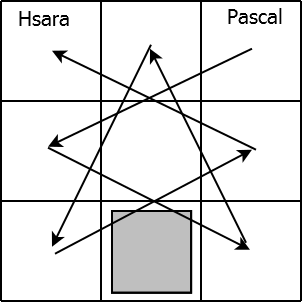
\includegraphics[width=0.25\textwidth]{hestar.png}
\caption{An illustration of Sample Input 2 showing how Pascal can jump to reach Hsara.}
\label{overflow}
\end{figure}

\section*{Scoring}
Your solution will be tested on a set of test groups. To earn points
for a group, you must pass all test cases in that group.

\begin{tabular}{| l | l | l | l |}
\hline
Group & Points & Constraints \\ \hline
1 & 40 & $3 \le N,M \le 100$ \\ \hline
2 & 60 & $3 \le N,M \le 500$ \\ \hline
\end{tabular}
